% diagrams/english/arbol-otono.tex -- el árbol de otoño del dibujo de
% Lucía, para "Read and colour": el tronco, la copa, el sol que asoma
% detrás y la hierba, cada parte cerrada para colorearla. La copa es una
% nube: círculos rellenos de blanco y, encima, otros un poco más
% pequeños que borran las curvas de dentro -- solo queda el contorno.
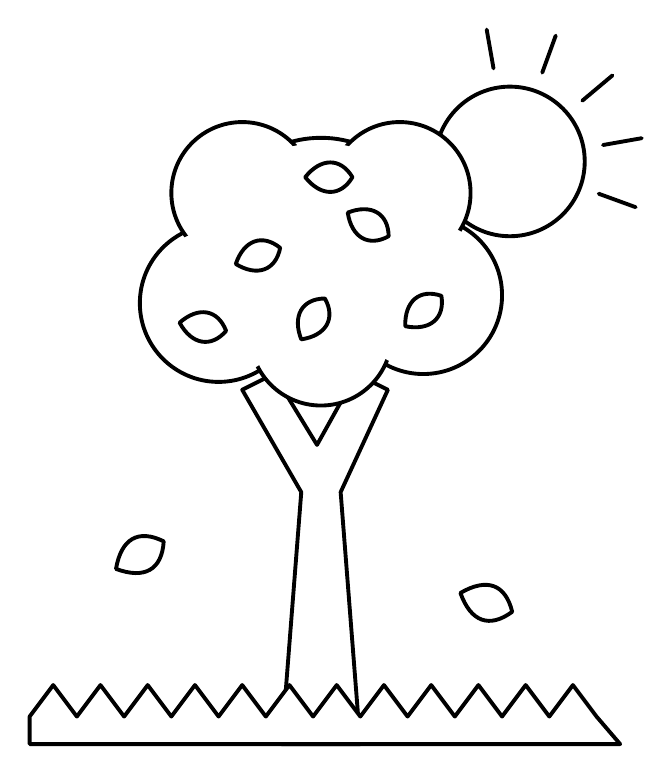
\begin{tikzpicture}[line width=1.4pt, line cap=round, line join=round, scale=1.0]
  % el sol, detrás de la copa
  \filldraw[fill=white] (5.5,7.4) circle (0.95);
  \foreach \a in {-20,10,40,70,100} {
    \draw (5.5,7.4) ++(\a:1.2) -- ++(\a:0.5);
  }
  % el tronco, con dos ramas que se meten en la copa
  \filldraw[fill=white] (2.6,0) -- (2.85,3.2) -- (2.1,4.5) -- (2.5,4.7) -- (3.05,3.8)
    -- (3.55,4.7) -- (3.95,4.5) -- (3.35,3.2) -- (3.6,0) -- cycle;
  % la copa
  \foreach \x/\y/\r in {3.1/6.3/1.4, 1.8/5.6/1.0, 4.4/5.7/1.0, 2.1/7.0/0.9,
                        4.1/7.0/0.9, 3.1/5.2/0.9} {
    \filldraw[fill=white] (\x,\y) circle (\r);
  }
  \foreach \x/\y/\r in {3.1/6.3/1.4, 1.8/5.6/1.0, 4.4/5.7/1.0, 2.1/7.0/0.9,
                        4.1/7.0/0.9, 3.1/5.2/0.9} {
    \fill[white] (\x,\y) circle (\r-0.06);
  }
  % unas hojas dentro de la copa, para que se vea que son hojas
  \foreach \x/\y/\g in {2.3/6.2/20, 3.7/6.6/-30, 3.0/5.4/60, 1.6/5.3/-10, 4.4/5.5/40, 3.2/7.2/0} {
    \begin{scope}[shift={(\x,\y)}, rotate=\g]
      \draw (-0.3,0) .. controls (-0.1,0.25) and (0.15,0.25) .. (0.3,0)
        .. controls (0.15,-0.25) and (-0.1,-0.25) .. (-0.3,0) -- cycle;
    \end{scope}
  }
  % dos hojas que caen
  \foreach \x/\y/\g in {0.8/2.4/30, 5.2/1.8/-20} {
    \begin{scope}[shift={(\x,\y)}, rotate=\g]
      \filldraw[fill=white] (-0.35,0) .. controls (-0.1,0.3) and (0.15,0.3) .. (0.35,0)
        .. controls (0.15,-0.3) and (-0.1,-0.3) .. (-0.35,0) -- cycle;
    \end{scope}
  }
  % la hierba
  \filldraw[fill=white] (-0.6,0) -- (-0.6,0.35)
    \foreach \x in {-0.3,0.3,...,6.9} { -- (\x,0.75) -- (\x+0.3,0.35) } -- (6.9,0) -- cycle;
\end{tikzpicture}
